\chapter{Current State}
\label{chapter:current-state}

The instrument was installed in November and December 2024, and we are still working to optimize its performance. The current state of the instrument and its associated systems is as follows:

\begin{figure}
\centering
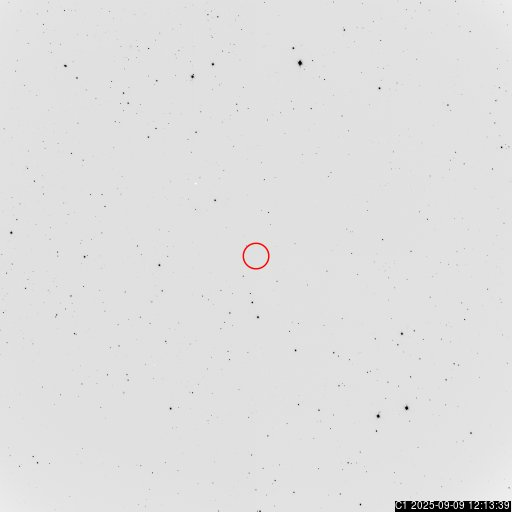
\includegraphics[width=0.65\linewidth]{figure/C1.jpg}

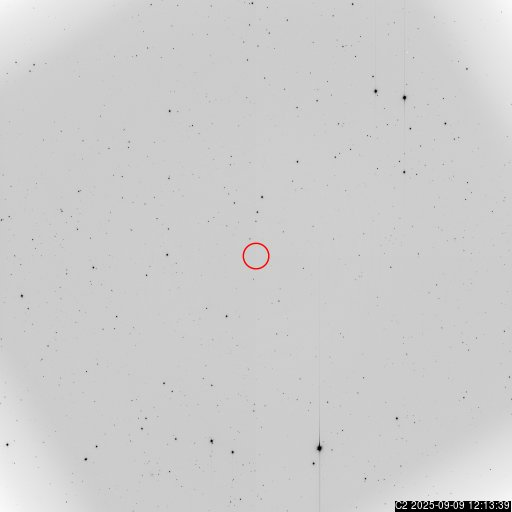
\includegraphics[width=0.65\linewidth]{figure/C2.jpg}

\caption{Typical images in the blue channel (above) and red channel (below). Note that the red channel is flipped vertically with respect to the blue channel because of the reflection off the second dichroic. Note also the vignetting in the red channel caused by the incorrect orientation of the filters and the trails above and below bright stars.}
\label{figure:typical-images}
\end{figure}

\begin{itemize}

\item 
The blue channel is operational and works as expected. 

\item 
The red channel is operation and works largely as expected. However:

\begin{itemize}
    \item Compared to the blue CCD, the red CCD shows worse artifacts above and below bright sources, and we anticipate working with the vendor to tune the CCD voltages and improve this.
    \item There is vignetting in the corners of the red CCD as the filter wheel has an incorrect rotation. We hope to correct this in November 2025.
\end{itemize}

Both of these problems can be seen in Figure~\ref{figure:typical-images}.

\item 
The telescope is operational and working largely as expected. However: 

\begin{itemize}
    \item We have not completed optical alignment of the telescope. As a result of this, we see field-depended comma in both detectors. Nevertheless, the instrument has given images with FWHM of 0.8 arcsec in the center of the field, but the FWHM is worse away from the field center. We hope to complete alignment in November 2025.
    \item The telescope tracking is not as good as we anticipated; although short exposures often have a FWHM of less than 1.0 arcsec, exposures of sixty seconds typically have a FWHM of about 1.2 arcsec. We will work in September 2025 to improve the pointing map and hence the tracking.
\end{itemize}

\item
The automatic data-processing pipeline is not yet available. We still do not have a date for when it will be available. 

However, we have an engineering pipeline that is capable of stacking images and doing a simple sky subtraction. It requires some manual tuning (selecting a star for alignment and determining the fraction of frames to reject). It does not perform astrometric or photometric calibration or produce source catalogs. If you are interested in this pipeline, please contact Alan Watson <\href{mailto:alan@astro.unam.mx}{alan@astro.unam.mx}> directly.

\item
The scheduler is not yet fully integrated. Observations have to be programmed by hand, which limits flexibility and favors blocks that are simpler to program.

\end{itemize}
